\section{Introduction}

\section{Background}

\section{Experimental}
The experimental results and procedures presented here will
focus on those nanowires derived from Bi\textsubscript{2}Te\textsubscript{3} catalytic seeds
deposited on pristine (0001) sapphire substrates. The results
obtained will then be compared to the CdTe nanowires,
described elsewhere [19], obtained using bismuth catalytic
seeds deposited on alcohol-altered (0001) sapphire substrates.The experimental results and procedures presented here will
focus on those nanowires derived from Bi\textsubscript{2}Te\textsubscript{3} catalytic seeds
deposited on pristine (0001) sapphire substrates. The results
obtained will then be compared to the CdTe nanowires,
described elsewhere [19], obtained using bismuth catalytic
seeds deposited on alcohol-altered (0001) sapphire substrates.

The Bi\textsubscript{2}Te\textsubscript{3} seeds were prepared using the PLD process
(GSI Lumonics IPEX-848 excimer laser, \textlambda~= 248 nm, laser
energy density = 2 J cm\textsuperscript{-2} , laser spot size = 1.2$\times$1.2 mm\textsuperscript{2}).
The target used was prepared in-house from commercially
available Bi\textsubscript{2}Te\textsubscript{3} pieces (99.999\% purity). These pieces were
melted in a cylindrical graphite mould that was machined to
sizes able to yield a 1 inch target weighing approximately 10 g. This procedure was carried out in an argon background gas. Prior to the deposition, the sapphire substrate was heated to 
400\degree\celsius and held there for 10 min in an oxygen background 
pressure of 300 mTorr.The substrate was then cooled to room temperature where a 20 \AA thick film of Bi\textsubscript{2}Te\textsubscript{3} was deposited. This deposition lasted 35 s at a laser repetition rate of 3 Hz. 
Once deposited, the film was then heated to 370\degree\celsius where, over 
the course of 10 min, it would dewet forming Bi\textsubscript{2}Te\textsubscript{3} 
seeds. At this point, a 30 sccm helium flow was introduced 
into the chamber such that the pressure was maintained at 
400 mTorr. Material from a rotating CdTe target, grown using 
the Bridgman method, was then ablated onto the substrate for 
time intervals typically in the range of 30?45 min at a laser 
repetition rate of 8 Hz. The nanowires were then allowed to 
cool to room temperature in the helium ambient.

\section{Results and Discussion}
Figure 1 shows an SEM image, of the Bi\textsubscript{2}Te\textsubscript{3}
catalytic seeds formed on the (0001) sapphire substrate. The
seeds show a substantial size distribution with diameters
as large as 150 nm. While these seeds show enhanced
stability, they are still prone to evaporation and will disappear
completely if the CdTe deposition is delayed by approximately
10 min. As was the case for the bismuth catalysts, the Bi\textsubscript{2}Te\textsubscript{3}
seeds gain stability from exposure to the cadmium/tellurium
flux. It is also likely that the seeds shown in the image
are somewhat different from those available when nanowire
growth commences as the time required to cool these seeds
to room temperature provided ample opportunity for further
evaporation and Ostwald ripening.
\begin{figure}
    \centering
    \begin{subfigure}[t]{0.5\textwidth}
        \centering
        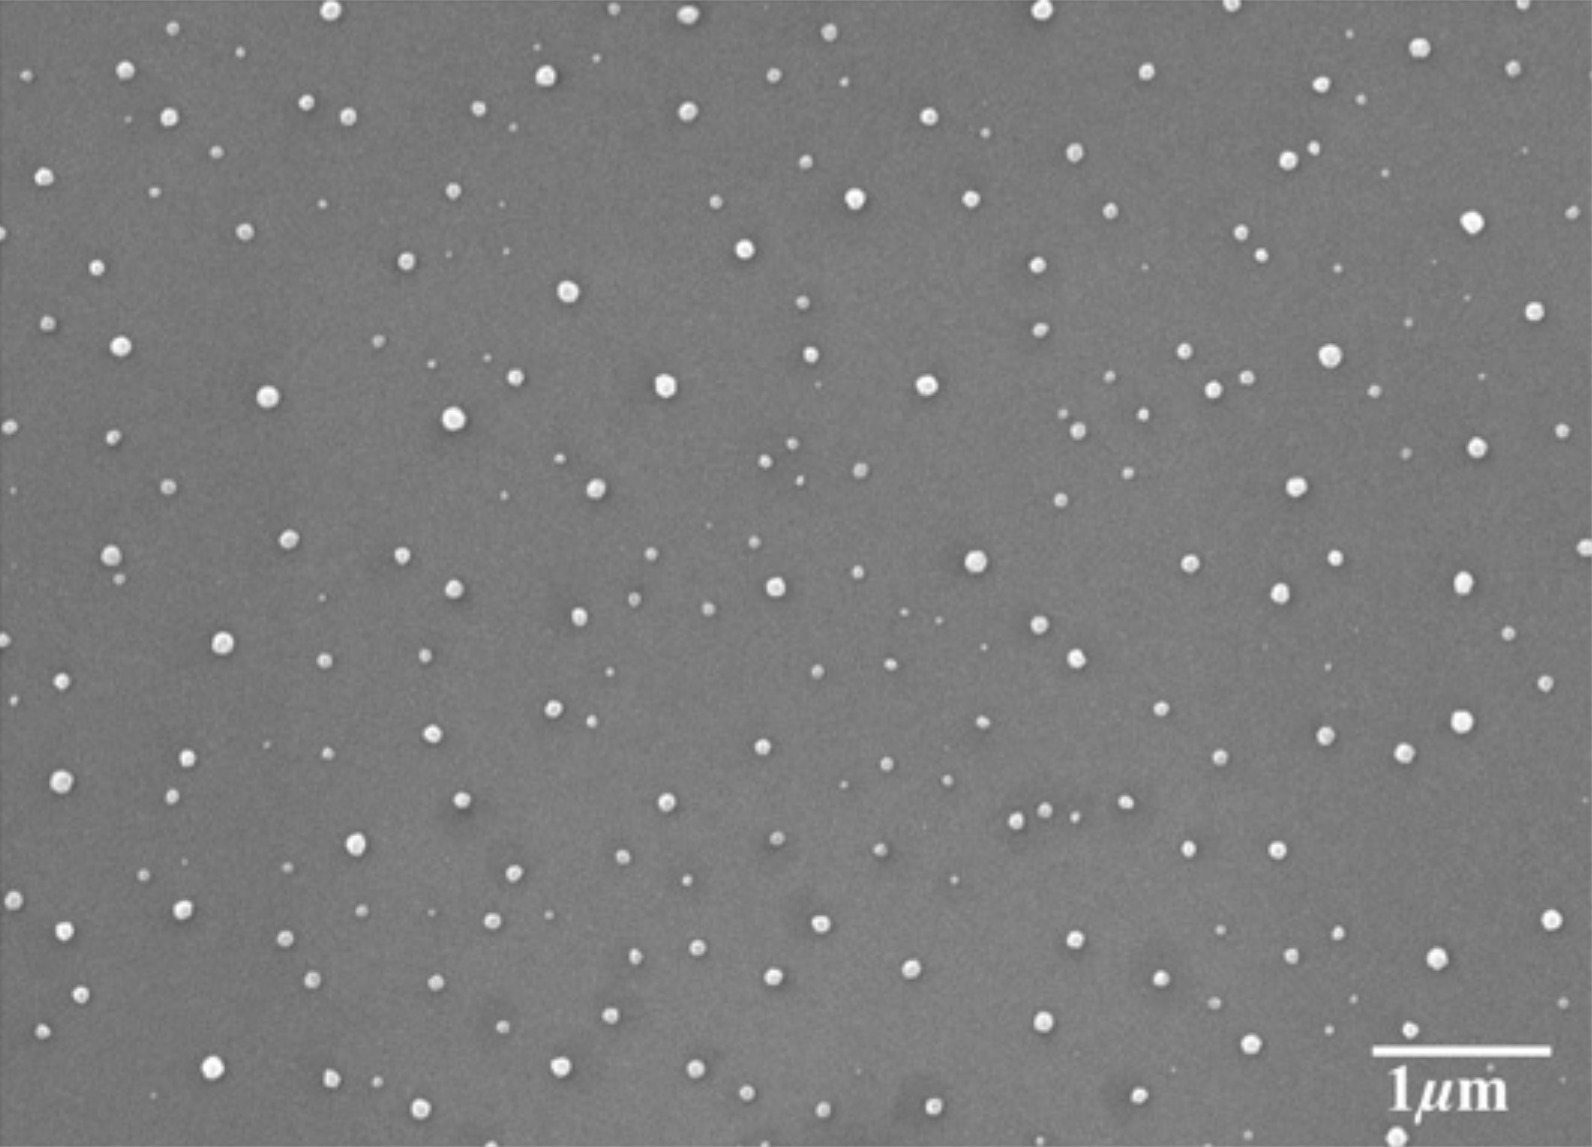
\includegraphics{nanocdte_bite}
        \caption{\label{fig:nanocdte_bite}SEM image of the Bi2 Te3 seeds that were used as catalysts 
            for CdTe nanowires.}
    \end{subfigure}%
    \begin{subfigure}[t]{0.5\textwidth}
        \centering
        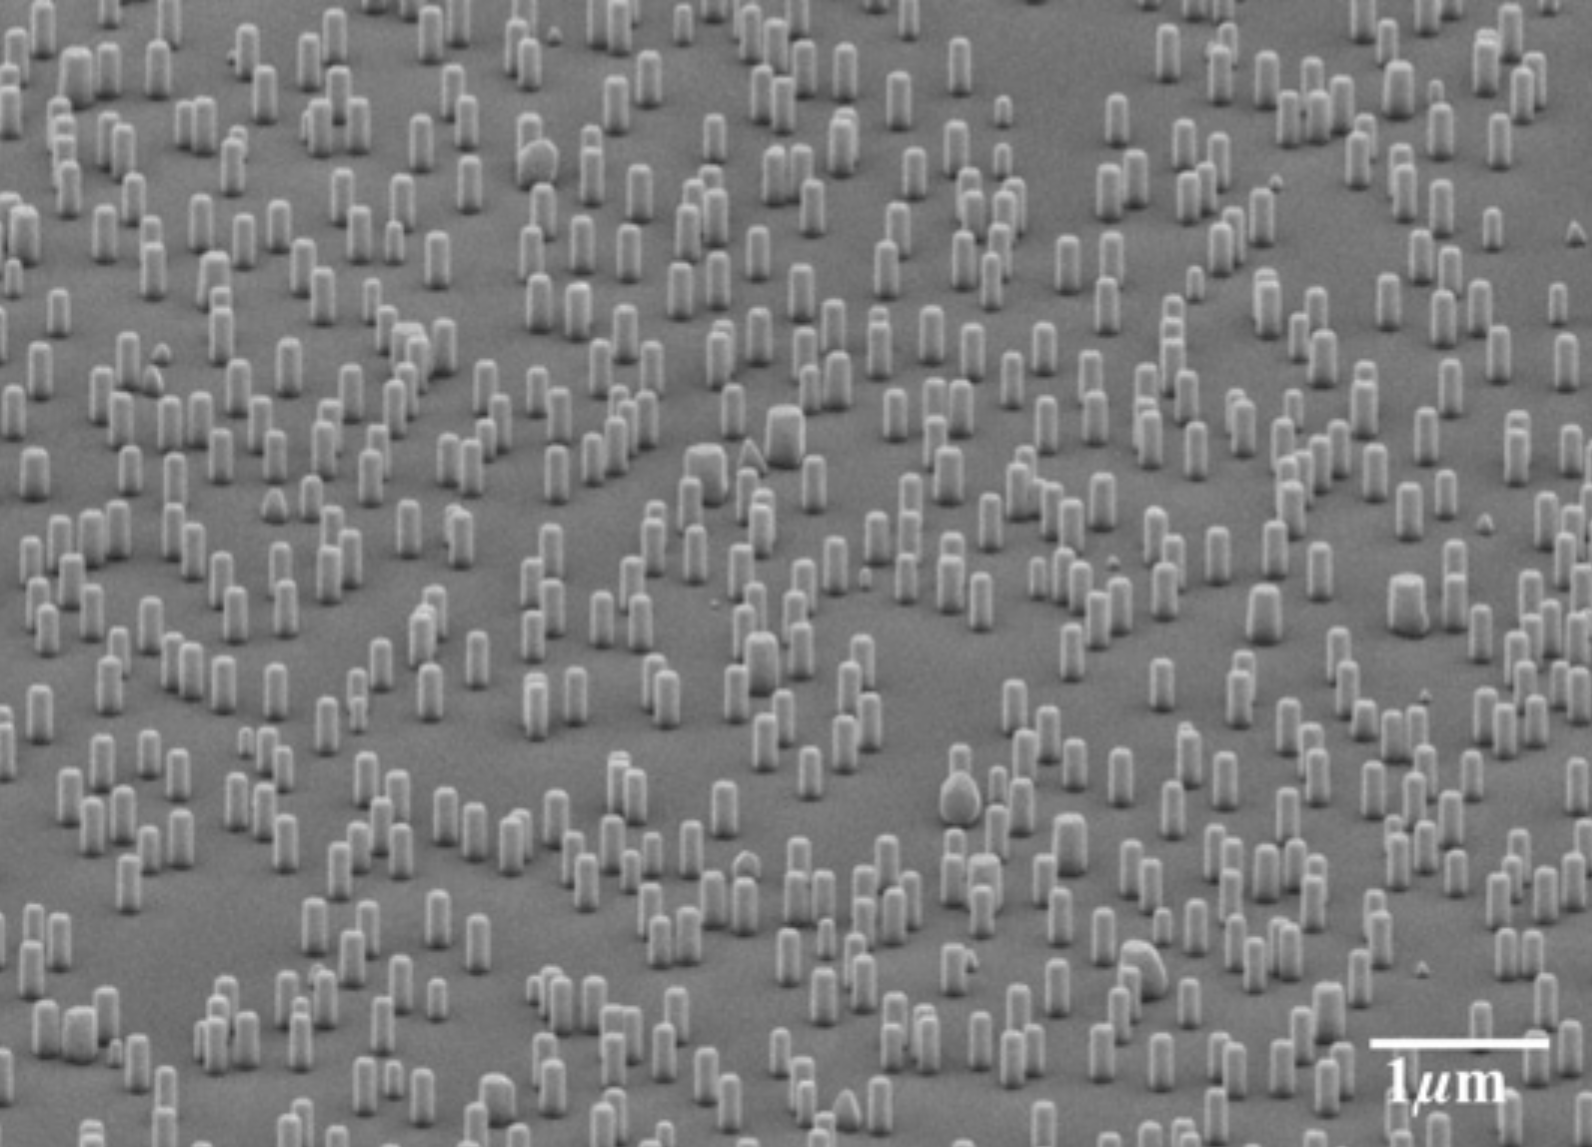
\includegraphics{nanocdte_nanowires}
        \caption{\label{fig:nanocdte_nanowires} SEM image of CdTe nanowires derived from Bi2 Te3
            catalytic seeds presented from a 70\degree~tilt side view.}
    \end{subfigure}
    \caption{\label{fig:nanocdte_sem}SEMs of seeds and resulting wires}
\end{figure}

Figure 2 shows an SEM image of the CdTe nanowires
derived from Bi\textsubscript{2}Te\textsubscript{3} seeds. In many respects, these nanowires
are indistinguishable from those grown using bismuth seeds
in conjunction with an alcohol-altered surface [19]. The two
methods both yield vertically aligned nanowires that are highly
faceted, share an epitaxial relationship with the substrate and
grow without a two-dimensional planar layer. The nanowires
are identical from a structural standpoint as well, exhibiting
the wurtzite crystal structure instead of the bulk zinc blende phase. Figure 3
shows a pole figure that includes contributions from both
the (111) zinc blende and (0002) wurtzite planes. Both phases give rise to a peak in the
centre of the pole, but a zinc blende phase must also give rise to
a ring of three peaks at the outer extent of the pole. For the pole
figure shown no such peaks are observed, but in general a small
zinc blende signature was visible. The three small peaks that
do appear in the pole figure are associated with the sapphire
substrate.
\begin{figure}
    \centering
    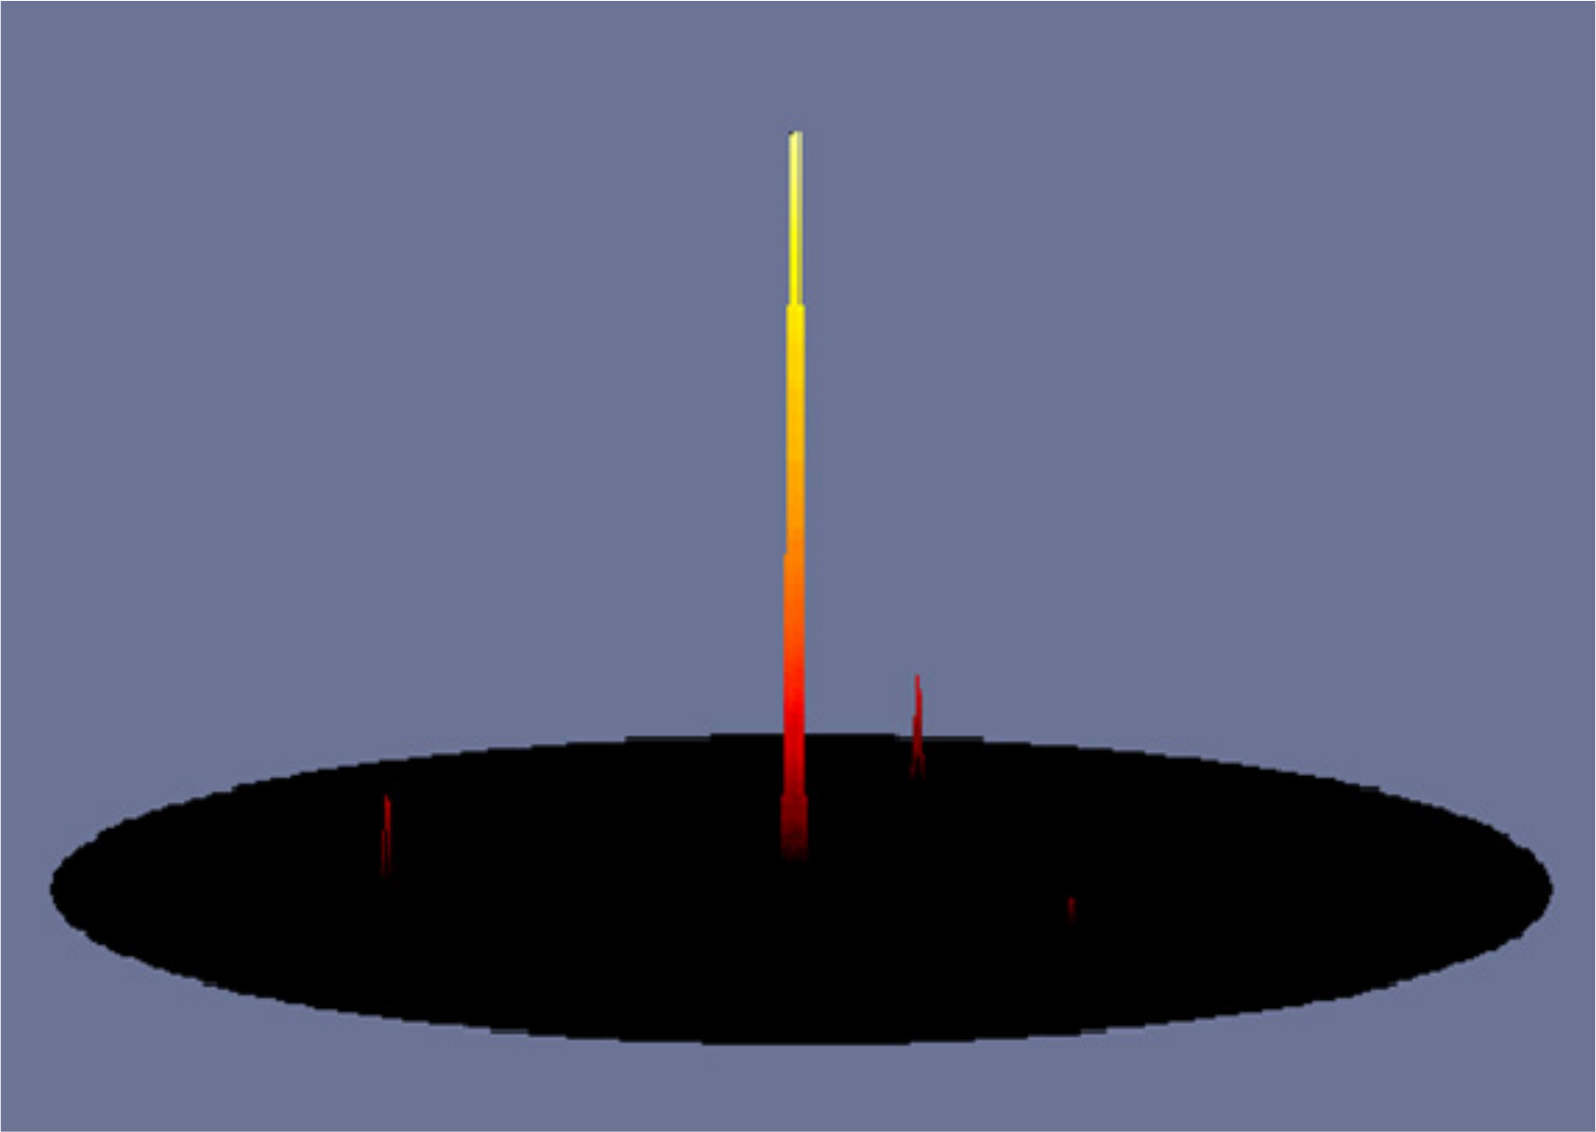
\includegraphics{nanocdte_polefigure}
    \caption{\label{fig:nanocdte_polefigure}CdTe pole figure results for 2\straighttheta~values that include contributions from both the (111) zinc blende and (0002) wurtzite phases. The pole figure shows no evidence of a zinc blende phase. The three small peaks originate from the (0001) sapphire substrate.}
\end{figure}

Even though these Bi\textsubscript{2}Te\textsubscript{3} catalysed nanowires share
many similarities with those derived from the bismuth seeds
deposited on an alcohol-altered surface, there do exist
substantial differences. One of the most striking differences
is the nanowire size distribution observed in the SEM images
of figure 4. This size distribution is quantified by the colour
map presented in figure 5(a). It shows a nanowire height
versus diameter distribution for the Bi\textsubscript{2}Te\textsubscript{3} seeded nanowires. It is quite clear from the map that larger diameter nanowires exhibit higher axial growth rates than smaller diameter ones. Figures 5(b) shows the same distribution for nanowires derived 
from bismuth seeds deposited on an alcohol-altered surface. A 
comparison of the two colour maps shows that the alcohol- 
altered surface gives rise to a significantly narrower size 
distribution. It is also apparent from the distributions that the 
Bi\textsubscript{2}Te\textsubscript{3} seeded nanowires are of larger diameter with values typically in the range of 80?200 nm. Also different is the fact that the nanowire height is not limited to 300 nm. Instead the nanowires grow longer while at the same time exhibiting
substantial growth in the lateral direction (figure 6).
Moving away from the optimum growth conditions gives
rise to other significant differences between the two nanowire
growth procedures. First, nanowires formed at the substrate's
edge have slanted tops where the direction of the slant at the
left and right edges of the substrate point in opposite directions
(figure 7). Also of note is the fact that the nanowire's cross-
section is no longer hexagonal, but instead elongates along the
direction of the slant. Second, at high growth rates Bi\textsubscript{2}Te\textsubscript{3}
seeded nanowires show significant tapering (figure 8).
\begin{figure}
    \centering
    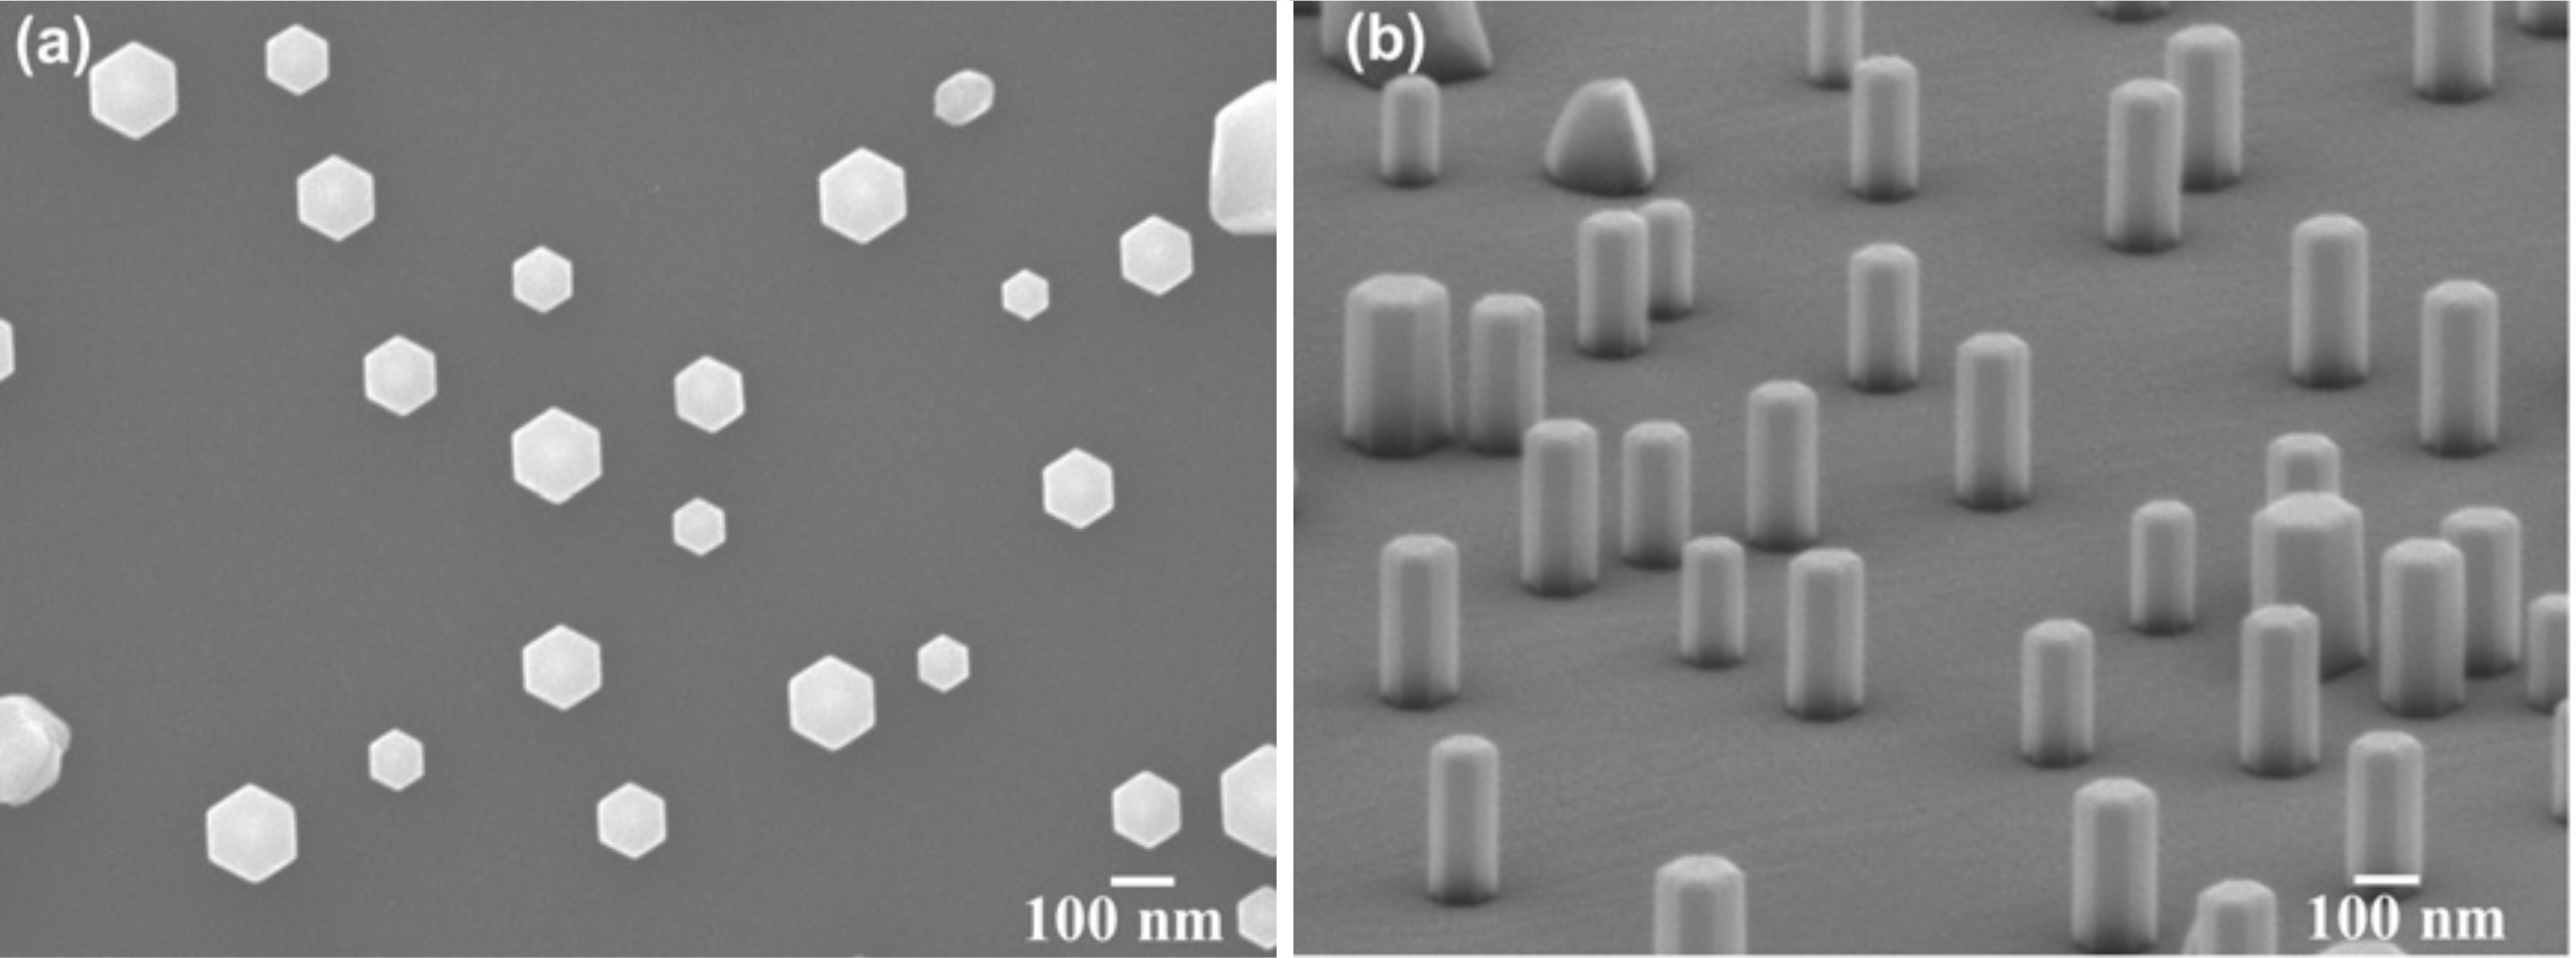
\includegraphics[width=\textwidth]{nanocdte_SEM2}
    \caption{\label{fig:nanocdte_SEM2}SEM images of CdTe nanowires from a (a) top and (b) side view (70\degree~tilt). Note that the highly faceted wires exhibit a substantial variation in both heights and diameters.}
\end{figure}
\begin{figure}
    \centering
    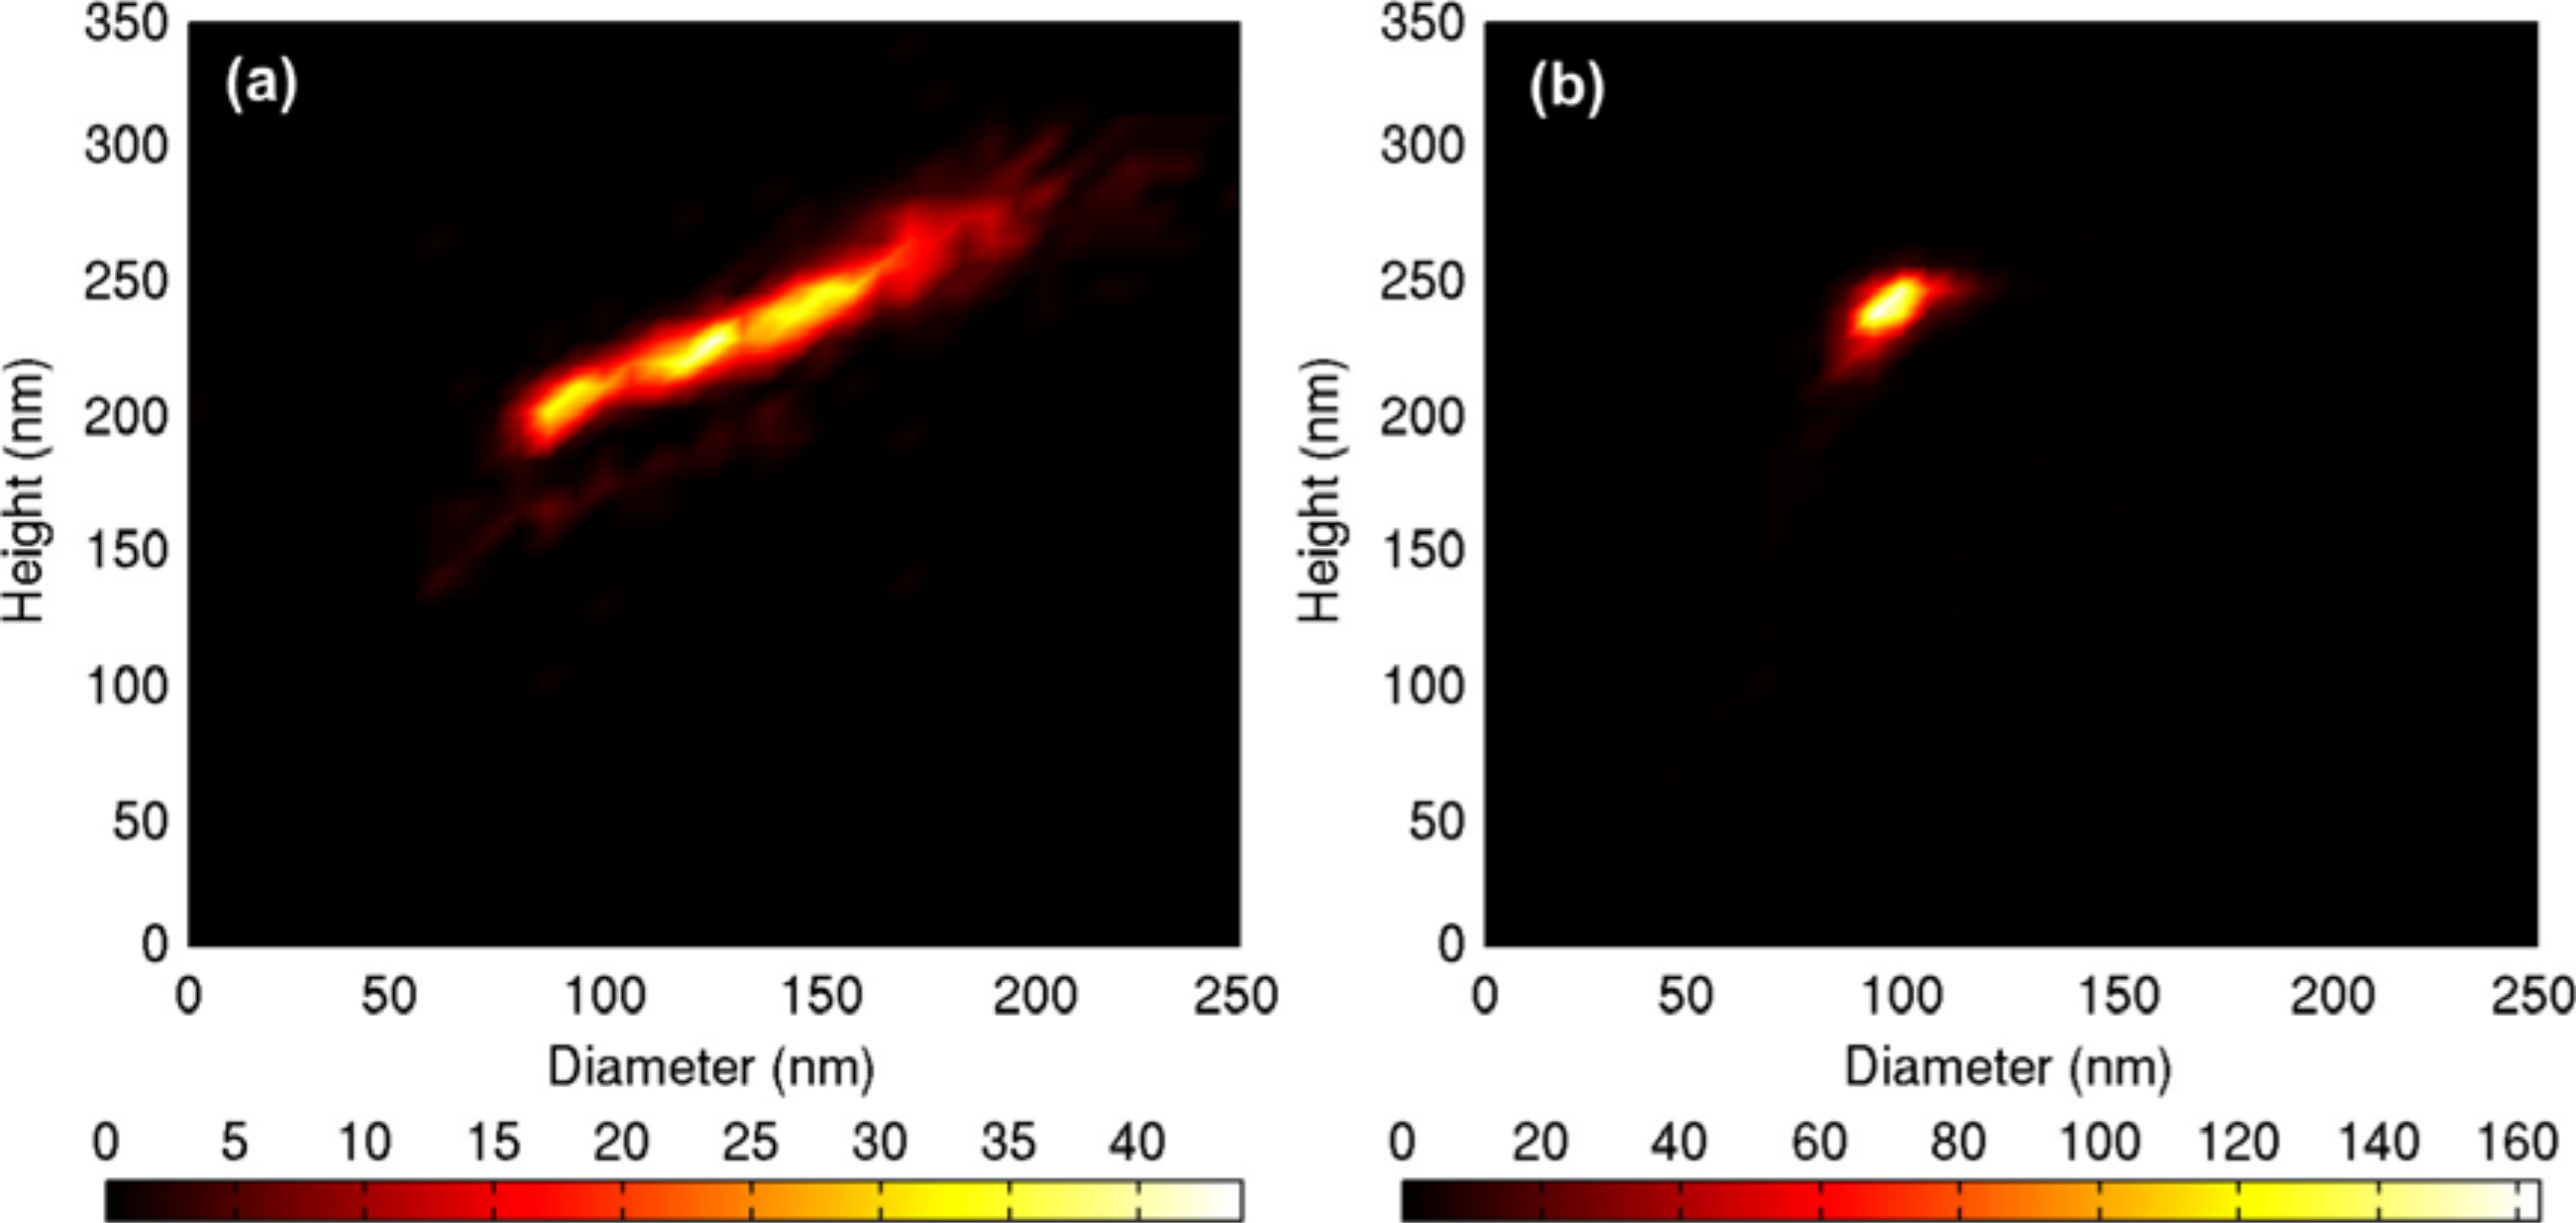
\includegraphics[width=\textwidth]{nanocdte_stats}
    \caption{\label{fig:nanocdte_stats}Colour map showing the nanowire height versus diameter size distribution for nanowires derived from (a) Bi\textsubscript{2}Te\textsubscript{3} catalytic seeds
        and (b) bismuth seeds deposited on an alcohol-altered surface. The maps were generated from the measured dimensions of (a) 1344 and
        (b) 966 nanowires. The colour bar below each figure denotes the number of times a nanowire of a given dimension is observed. Note that the
        Bi\textsubscript{2}Te\textsubscript{3} seeded nanowires exhibit a broader size distribution and sizes that are, in general, larger than the bismuth seeded wires.}
\end{figure}
\begin{figure}
    \centering
    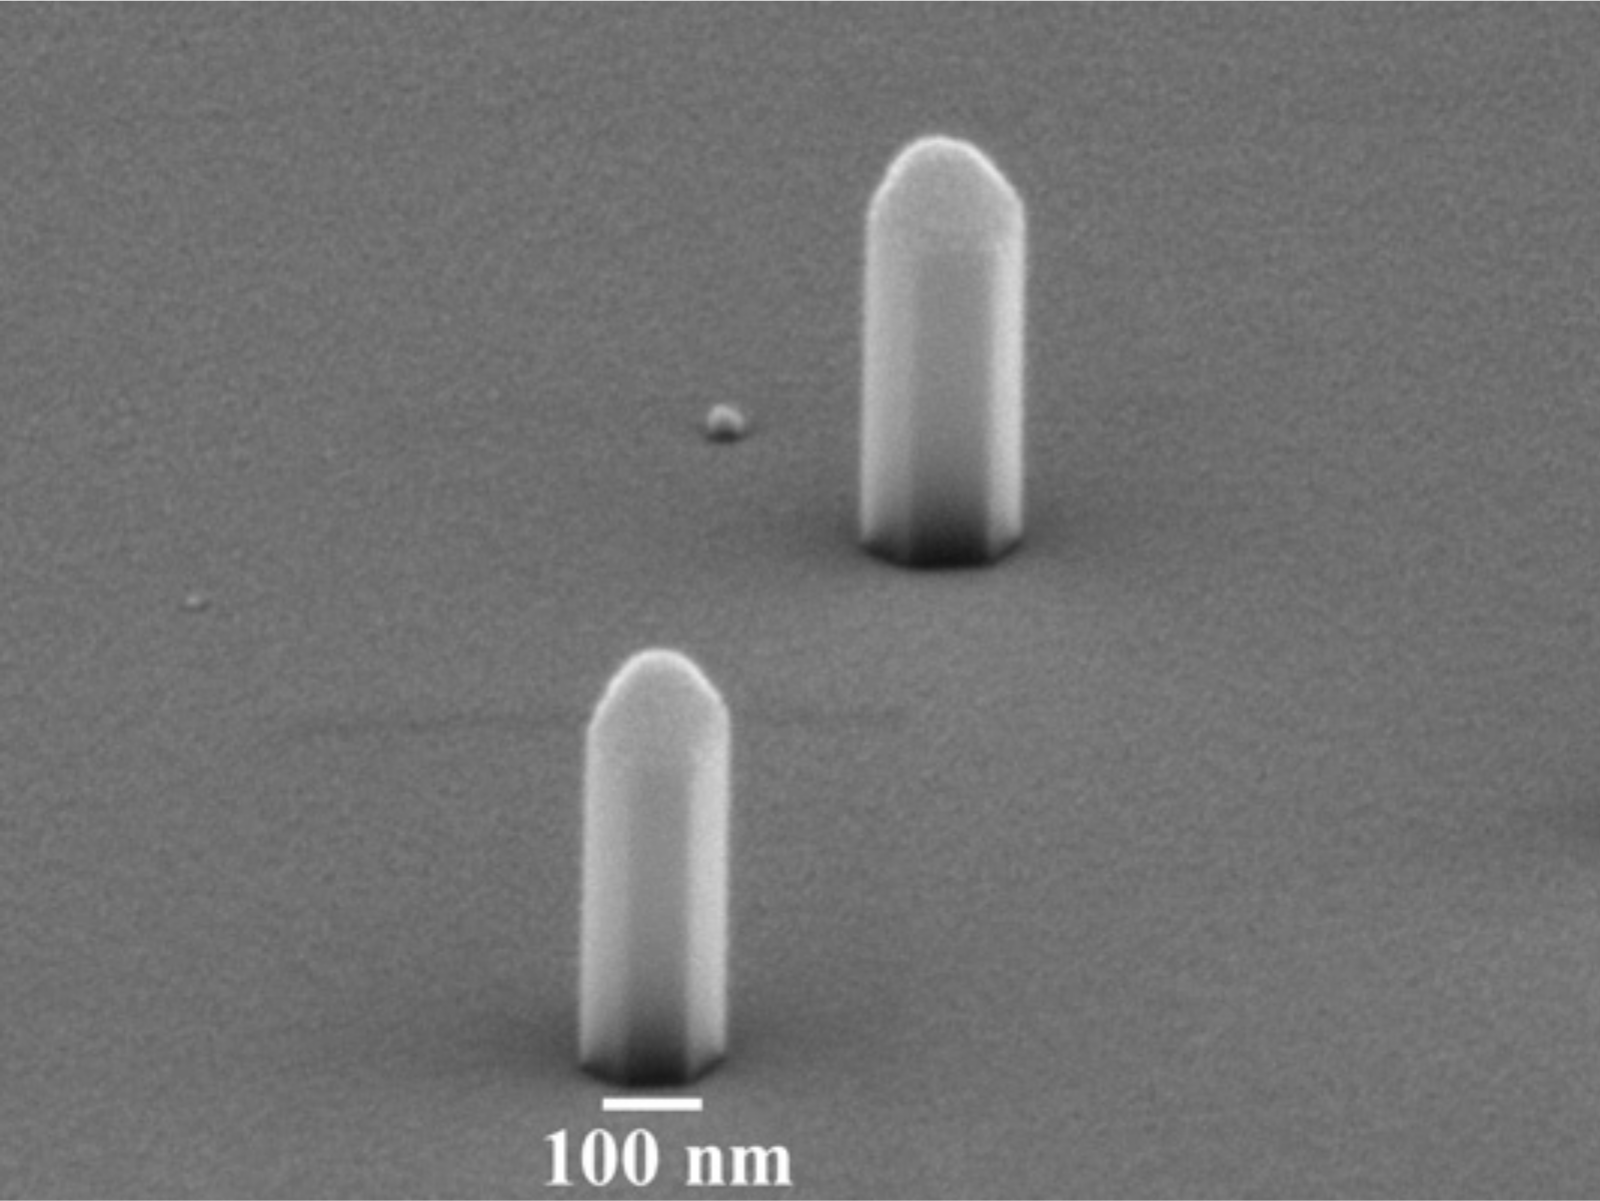
\includegraphics{nanocdte_lateral}
    \caption{\label{fig:nanocdte_lateral}SEM images of CdTe nanowires deposited using extended 
        growth times where increases to the height are met with substantial lateral growth.}
\end{figure}
\begin{figure}
    \centering
    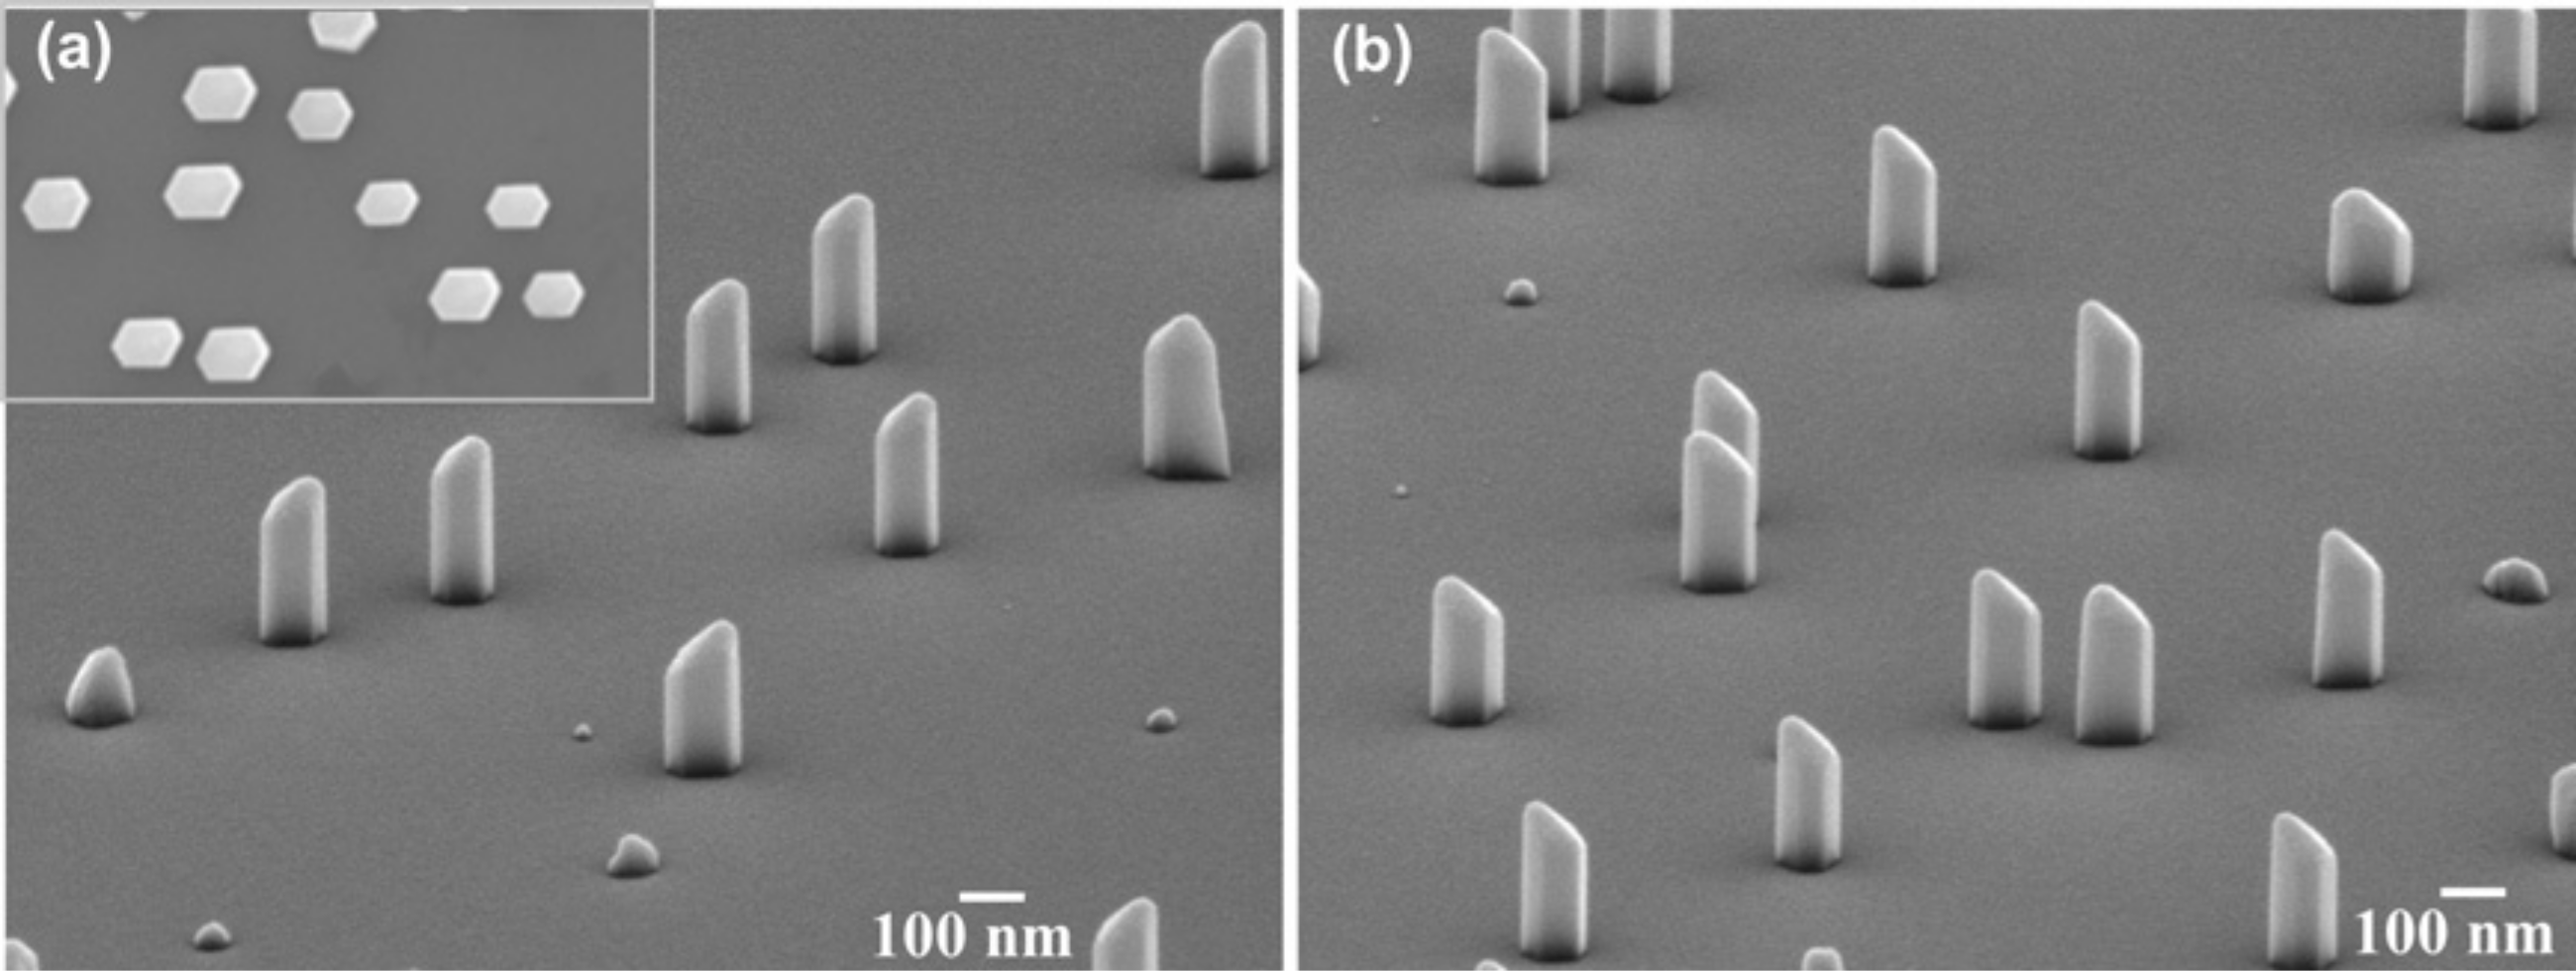
\includegraphics{nanocdte_slanted}
    \caption{\label{fig:nanocdte_slanted}SEM images of CdTe nanowires with slanted tops that have formed at the (a) left and (b) right edge of the substrate. Note that the
        tilt is in opposite directions. The top views of these nanostructures, shown in the inset to (a), indicate that the hexagonal cross-sections are
        elongated in the horizontal direction.}
\end{figure}
\begin{figure}
    \centering
    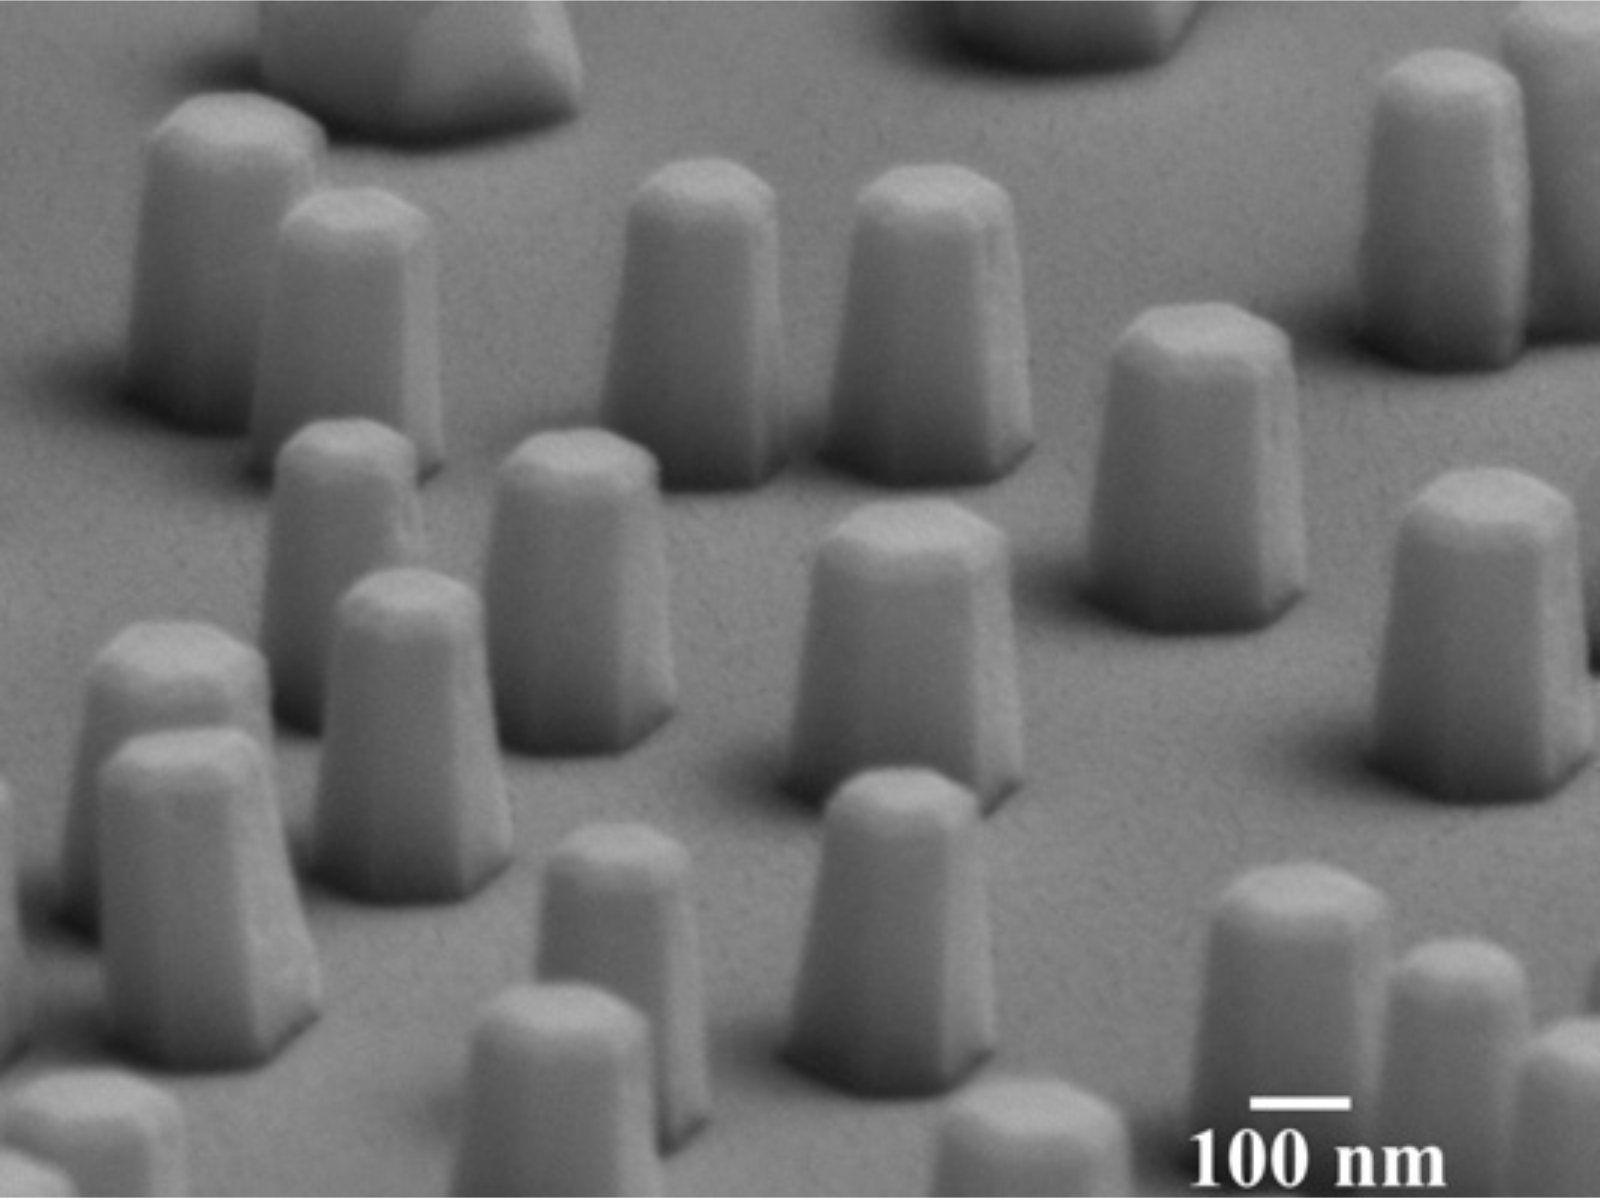
\includegraphics{nanocdte_tapered}
    \caption{\label{fig:nanocdte_tapered}SEM image showing tapered CdTe nanowires.}
\end{figure}
This work combined with our previous results has demon-
strated that CdTe nanowire structures can originate from cat-
alytic seeds derived from two separate processes, with each
of these processes having advantages and disadvantages. Bis-
muth seeds, in combination with an alcohol-altered surface,
give rise to superior nanowire uniformity, but there exist
nanowire height limitations and fabrication can only proceed
using volatile catalytic seeds maintained in a narrow window
of processing parameters. The Bi\textsubscript{2}Te\textsubscript{3} seeds are much more stable at the temperatures needed to initiate CdTe nanowire growth. This makes nanowire production possible without the
cumbersome alcohol pre-treatment of the substrate's surface.
The main disadvantage is that the nanowire size and shape distributions are severely compromised.

It is important to emphasize that well over one hundred
samples have been characterized for each of the two nanowire
deposition methods. As a result, nanowire fabrication has
been attempted over a broad range of growth conditions.
Thus, the features presented here as unique to the Bi\textsubscript{2}Te\textsubscript{3}
initiated nanowires have been shown to decisively differentiate
themselves from those observed using bismuth seeds deposited
on an alcohol-altered surface. If, as expected, both the bismuth
and Bi\textsubscript{2}Te\textsubscript{3} catalytic seeds assume the same composition once
exposed to a flux of cadmium and tellurium then the differences
observed between the two methods must be attributed to the
presence or absence of an alcohol-altered substrate surface. It
is our conjecture that this can be done within the confines of
the existing nanowire growth modes.

For both nanowire deposition methods the catalytic
seeds are derived from a thin film that dewets at elevated
temperatures. Once formed, these seeds are subject to Ostwald
ripening, where there is an exchange of atoms along the
substrate's surface with larger seeds growing at the expense
of smaller ones [21, 22]. The effectiveness of this process is
governed by the adatom's surface diffusion length given by
the square root of the product of its diffusion coefficient and
lifetime. If this length is larger than the separation between
seeds then Ostwald ripening proceeds in the usual manner
where, as time progresses, there exists an increasing variation
in seed size. On the other hand, if this length is reduced
to where atoms liberated from one seed evaporate before
encountering a second one, then a narrow size distribution will
be maintained, but accompanied by a continuous reduction in
the seed's diameter.

It is clear from our results that the pristine substrate used
for the Bi\textsubscript{2}Te\textsubscript{3} seeds leads to sufficient surface mobility for
Ostwald ripening to broaden the distribution of seed diameters.
Due to the higher volatility of tellurium we expect that this
ripening process will result in bismuth-rich seeds. Indeed, the
binary phase diagram indicates that the growth temperature is
too low for the seeds to melt unless there is first a substantial
loss of tellurium [23]. The combination of Ostwald ripening in conjunction with evaporation leads to bismuth-rich catalytic
seeds of different sizes which in turn give rise to nanowires of
varying diameters. Corrupting the surface with alcohol alters
this process by dramatically reducing the surface mobility; this
increases the lifetime of the seed on the surface and frustrates
the Ostwald ripening process, i.e., any bismuth atoms liberated
from an individual seed are backscattered to the original seed
or evaporate from the surface before reaching a second seed.
With the ripening process halted, the distribution of seed
diameters remains narrow, ultimately giving rise to a narrow
distribution of nanowires.

With the catalytic seeds in place and exposed to a
flux of cadmium and tellurium atoms it is expected that
both the bismuth and Bi\textsubscript{2}Te\textsubscript{3} seeds will evolve to the same
ternary composition. While the ternary phase diagram for
the cadmium/tellurium/bismuth system is unknown, it is well
established that individually both tellurium and cadmium are
soluble in bismuth [23]. The catalytic seed's ability to stabilize
both elements on the timescales necessary for CdTe formation
is crucial. This is made evident by the fact that the CdTe
nanowires grow in the absence of a two-dimensional planar
layer. This is attributable to the fact that both cadmium and
tellurium have negligible sticking coefficients at the substrate
temperature used. It is only through the formation of CdTe
that these species have significant lifetimes on the substrate's
surface. For the growth conditions used, however, the adatom
lifetimes are too small to enable CdTe formation directly on the sapphire negating a planar growth mode. As a result, CdTe growth can only proceed through the catalytically
driven process. Consistent with this analysis is a nanowire
height distribution with the tallest nanowires having the largest
diameters. This is in contrast to substrate-based nanowire
growth modes where the tallest nanowires are those with the
smallest diameters. For these systems, the nanowire height
distribution is driven by adatoms arriving at the substrate's
surface and making their way to the growth front via a random
walk that takes them up the nanowire's sidewalls. For the CdTe
case, the small adatom lifetime negates this process resulting
in a nanowire growth mode that is dependent upon the direct
impingement of atoms onto the catalytic seeds. Such a growth
mode is not commonly observed in semiconductor nanowire
systems.
\begin{figure}
    \centering
    \begin{subfigure}[t]{0.5\textwidth}
        \centering
        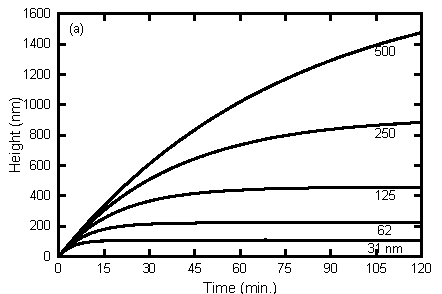
\includegraphics{nanocdte_model_thickness}
        \caption{\label{fig:nanocdte_model_thickness}}
    \end{subfigure}%
    \begin{subfigure}[t]{0.5\textwidth}
        \centering
        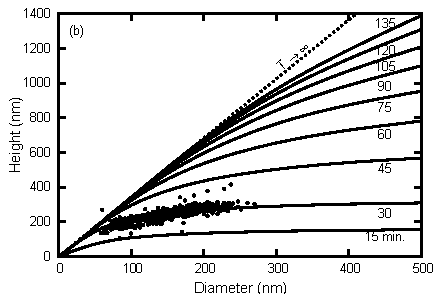
\includegraphics{nanocdte_model_time}
        \caption{\label{fig:nanocdte_model_time}}
    \end{subfigure}
    \caption{\label{fig:nanocdte_model}Simulation results showing (a) the time evolution of the nanowire height for the five labelled diameters and (b) time snapshots of the
        height versus diameter dependence for the times labelled. The dashed line shows the linear dependence expected when all nanowires reach an
        equilibrium condition. Superimposed over the simulation is the experimental data (black dots) of figure 5(a). The values used in this
        simulation have been scaled so as to fit this experimental distribution.}
\end{figure}

A growth mode driven by direct impingement, where all
the adatoms arrive normal to and are incorporated into the
nanostructure, will result in a nanowire height distribution
that is independent of diameter. There are, however, other
factors that can come into play. It has been demonstrated
both experimentally [24, 25] and theoretically [10, 13] that the
Gibbs?Thomson effect can give rise to a height distribution
directly proportional to the nanowire diameter. The effect
stipulates that the higher curvature associated with smaller
diameter seeds yields a higher effective vapour pressure,
reducing the uptake of atoms from the impinging vapour.
While this effect qualitatively gives rise to the observed CdTe
nanowire height distribution, it is unable to account for the
observed height limitation for the bismuth seeded nanowires
as it provides no means of halting the growth.

The self-limiting growth mode displayed by the bismuth
seeded nanowires deposited on an alcohol-altered surface
likely originates from an equilibrium that develops between the
addition of adatoms through direct impingement on the catalyst
and the loss of atoms from the sidewalls through sublimation.
The sublimation process is significant for the CdTe nanowires
as they will disappear completely in approximately 30 min if
left at the growth temperature in the absence of an incoming
flux of cadmium and tellurium atoms. A similar situation must
exist for the Bi\textsubscript{2}Te\textsubscript{3} seeded nanowires, but in this case the results are complicated by the distribution of the nanowires'
diameters and the lateral growth that becomes apparent for
long growth times. A stochastic simulation was conducted
to show the time evolution of the nanowires subject to a
sublimation process. With the uptake of material being
proportional to the area of the catalytic seed and the loss of
material being proportional to the area of the sidewalls, the
simulation yields nanowire heights showing the time evolution
presented in figure 9(a). Snapshots in time of the nanowire
height versus diameter distribution are shown in figure 9(b)
with the experimentally observed distribution of figure 5(a)
superimposed. The intent of this simulation was not to
rigorously model the nanowire growth as it ignores such factors
as the Gibbs?Thomson effect. It does, however, demonstrate
that sidewall sublimation limits nanowire height and results
in a size distribution qualitatively similar to that observed
experimentally.

Essential to this work is the observation that Bi\textsubscript{2}Te\textsubscript{3} seeded
nanowires show a marked tendency towards lateral growth,
while the bismuth seeded nanowires deposited on an alcohol-
altered substrate do not. This tendency is displayed not only
at long growth times, but also in the tapering shown at high
growth rates and in the elongation of the slanted-top nanowires
formed at the edge of the substrates. These three observations
are consistent with the preferential nucleation of adatoms at the
base of the nanowire where a weak nucleation site forms due to
atomic bonding from both the sidewall facet and the substrate.
Such a nucleation site would be analogous to the ones formed
on a vicinal substrate [26]. The atoms forming at the base
would then have to promote the propagation of a layer up the
nanowire's sidewall. The existence of a lateral growth mode
accounts for the formation of tall, large diameter nanowires
for extended growth times (figure 6). In the initial stages of
growth the axial growth rate exceeds the lateral growth rate by
a wide margin, but as the nanowire approaches its height limit
the axial growth slows dramatically as shown in figure 9(a).
The model presented, however, does not account for the
situation where a slow lateral growth mode accompanies the
axial growth. In this scenario, lateral growth results in larger
diameter nanowires which, in turn, allow for increased axial growth. As a result, both dimensions will grow slowly in
tandem provided that the catalytic material remains active as
it spreads out over the expanding top surface of the nanowire.

Lateral growth is most evident for the slanted-top
nanowires (figure 7) as it proceeds in an anisotropic manner.
In the PLD process cadmium and tellurium atoms exit the
target from an area a few square millimetres in diameter.
Thus, while the ablated material arrives normal to the centre
of the substrate, it arrives at an angle to the edges. As a
result, nanowires growing at the edges will have cadmium and
tellurium atoms preferentially landing on the sidewall facet
nearest to the centre of the substrate. Thus, the adatoms have
an increased likelihood of becoming a part of both the growth
front nearest to that sidewall facet as well as to any layer
propagating up that sidewall. It is this asymmetry that leads
to the anisotropic growth mode that is mirrored on opposite
sides of the substrate.

The extent of the lateral growth at the base of the nanowire
must be contingent upon the availability of adatoms on the
surface of the substrate. At slow growth rates the nucleation
of adatoms will be far more difficult as singly bonded atoms
and small clusters of atoms will easily dissociate, making
them prone to evaporation from the surface. At higher growth
rates the availability of adatoms increases allowing for larger
clusters to stabilize. Under these conditions the nanowires will
have a small, but significant, collection area. The effect of
this collection area, however, will diminish as one moves away
from the surface of the substrate, a situation that should give
rise to a tapered structure as shown in figure 8.

As previously mentioned, these lateral growth modes are
absent for the bismuth seeded nanowires deposited on an
alcohol-altered substrate. It is our conjecture that during the
dewetting process, the bismuth seeds are able to penetrate
through this surface-altered layer in a manner that effectively
cleans the surface and exposes the (0001) face of sapphire;
a face essential to the epitaxial alignment of the nanowires.
This statement is supported by the fact that a bismuth
absorption/desorption treatment has been used to remove
carbon-containing impurities from the surface of SrTiO3 and
LaAlO3 [27]. However, around the periphery of each seed it is
expected that the substrate's alcohol surface alteration persists.
As a result, the nucleation site at the base of the nanowire is of
poor quality as the substrate's epitaxial relationship no longer
exists due to the corrupted surface. It is this deterioration
in the nucleation site that inhibits the nanowire's ability to
grow laterally. In general, poor adhesion of adatoms to the
substrate should be quite detrimental to a lateral growth mode
as adatoms must already have a low probability of attaching to
the sidewall facet; if this were not the case a one-dimensional
nanowire growth mode would be unattainable. It should be
noted that the described process results in lateral overgrowth
suppression in a manner analogous to that used for nanowire
production through the use of selective area epitaxy. It is well
established that CdTe is prone to such a process as there exists
a substantive body of work detailing procedures for obtaining
selective epitaxy in the CdTe system [28-30]. Also supportive
of this explanation are reports detailing the fabrication of
vertically aligned nanowires, where non-vertically aligned
growth is eliminated through the use of organic layers [31-33].


\section{Implications for Symmetry and Energy at Epitaxial Surfaces}